%%% Preamble starts here.
\documentclass{amsart}
%for the heading
\usepackage{fancyhdr, enumerate}
%for the picture. 
\usepackage{tikz, calc}
%adjust the page width
\usepackage[margin=1in]{geometry}

%% The next line says how the "vertex" style of nodes should look: drawn as small circles.
\tikzstyle{vertex}=[circle, draw, inner sep=0pt, minimum size=6pt]
%%
%% Next, we make a \vertex command as a shorthand in place of \node[vertex} to get that style.
\newcommand{\vertex}{\node[vertex]}

\linespread{1.1}

%command for double parentheses
\newcommand{\textmultiset}[2]{\bigl(\!{\binom{#1}{#2}}\!\bigr)}
\newcommand{\displaymultiset}[2]{\left(\!{\binom{#1}{#2}}\!\right)}
\newcommand\multiset[2]{\mathchoice{\displaymultiset{#1}{#2}}
                                {\textmultiset{#1}{#2}}
                                {\textmultiset{#1}{#2}}
                                {\textmultiset{#1}{#2}}}

%special commands for number sets
\def\RR{{\mathbb R}}
\def\NN{{\mathbb N}}
\def\ZZ{{\mathbb Z}}
\def\QQ{{\mathbb Q}}
\def\CC{{\mathbb C}}

% header
\lhead{\sc  Combinatorics: Homework 12}
\chead{\sc Stefano Fochesatto} 
\rhead{\today}
\cfoot{}
\pagestyle{fancy}

%%%% Main document starts here.

\begin{document}
\thispagestyle{fancy}
 
\begin{enumerate}
%%%first problem
\item (Problem 6.4.1) True or False? (Justify your answer.)\\

(a) $n \rightarrow (a,b)$ if and only if $R(a,b) \leq n$\\

\textbf{answer:} True. This result was shown in reading question 259. The forwards proof basically boils down to the fact that every 2 coloring of a $K_{n}$ graph contains a 2 coloring of $K_{n-1}$ and hence if $n \rightarrow (a,b)$ it must be true that either $K_n$ is the smallest complete graph that is a Ramsey number for $R(a,b)$ or there is a subgraph with less vertices than $K_n$ that is also a Ramsey number for $R(a,b)$, hence $R(a,b) \leq n$. The backwards proof is essentially the same, if we know that $R(a,b) \leq n$ then $K_n$ must contain a subgraph $K_i$ where $n\geq i$ such that $R(a,b)  =  i$ and therefore there has to exist in every two coloring of $K_n$ a $K_a$ or $K_b$, thus $R(a,b) \leq n$.

\vspace{1in}

(b) $n \not\rightarrow (a,b)$ if and only if $R(a,b) \geq n$\\

\textbf{answer:} False. Simply because we know that for $R(a,b)  =  n$ it must satisfy two conditions, $n \rightarrow (a,b)$, and $n-1 \not\rightarrow (a,b)$. If $n \not\rightarrow (a,b)$ then we know right there that $R(a,b) \neq n$.\\

\vspace{1in}

(c) There is a red-blue coloring of $K_{300}$ with neither a red $K_6$ or a blue $K_7.$\\

\textbf{answer:} True. Our textbook contains a table of best know bounds on Ramsey numbers, and it says that for $R(6,7)  =  n$, $n$ is contained by $113 \leq n \leq 298$. Since $K_{300}$ is above our range, by problem $a$ it must contain either a red $K_6$ or a blue $K_7.$ \\

\vspace{1in}

(d) One way to determine an upper bound on $R(a,b)$ is to exhibit a coloring of a complete graph that has either a red $K_a$ or a blue $K_b.$\\


\textbf{answer:} False. It is not enough to show that one specific coloring of a complete graph satisfies a Ramsey problem. \\

\vspace{1in}

\item (Problem 6.4.3) Consider any five points in the plane such that no three lie on the same line. Prove that there exist four points that form the vertices of a convex quadrilateral.\\\\
Since any set of three collinear points forms a triangle, suppose we connect the three points such that we build the triangle that contains the most  possible points. There must exist a triangle that contains at least one vertex (PHP on 5 collinear points)  Then there are 2 cases.\\\\
Case 1; if there exists a point that is not enclosed by this triangle we are done and the convex quadrilateral is formed by the three chosen points and the point not enclosed.\\

\noindent Case 2: If both of the other points are enclosed by the triangle, then we can form a line with the interior points that splits the triangle into two. By PHP there must contain a side that contains two vertices of the triangle, and thus the convex parallelogram is formed by the interior points and the side of the triangle that contains two points. \\


\vspace{1in}

\item (Problem 6.4.5) Find a red-blue coloring of $K_{13}$ containing neither a red $K_3$ nor a blue $K_5.$\\
NOTE: It is not sufficient to simple draw a coloring. You need to explain why anyone would believe your drawing does not have a re $K_3$ or a blue $K_5.$\\\\
Consider the drawing of $K_{13}$ that starts with a $C_{13}$ on vertices labeled from $\{0,1,2,..,12\}$ then we select a vertex, say $0$ and we connect it to the vertex that is $5$ and $8$ away in the clockwise direction. Go around and do that for every vertex and we have colored all the red edges. The rest of the edges are blue. Suppose that there exists a $K_3$ or $K_5$ in our graph, If that is true it must also be true that there must exist a vertex that is a part of one of these graphs. Consider the following subgraph of our $K_{13}$ graph that focuses on the connectivity of $0$. By symmetry we can see that the connectivity of each vertex is the same ie wi
\begin{align*}
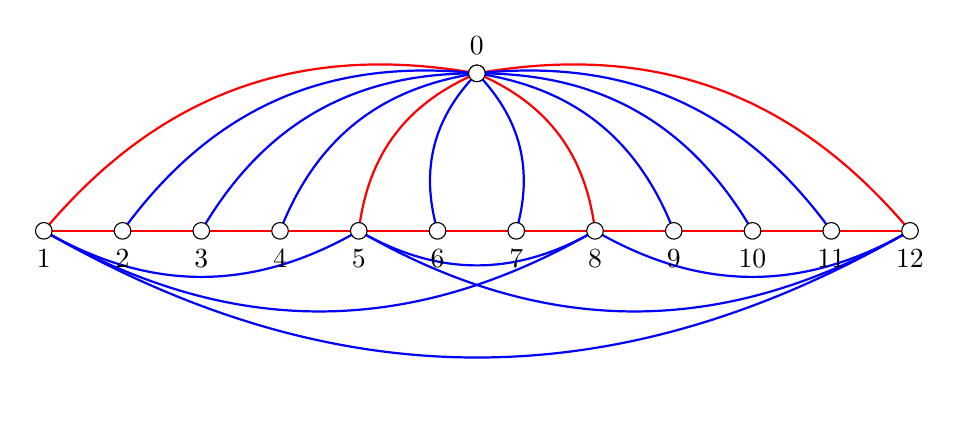
\begin{tikzpicture}[scale=1]
\foreach \i in {0,1,2,...,10}{\draw[thick, red] (\i,0) -- (\i+1,0);}
\vertex[fill=white] at (5.5,2) {};
\draw[thick, red] (5.5,2) to [bend right]   (0,0);
\draw[thick, red] (5.5,2) to [bend right]   (4,0);
\draw[thick, red] (5.5,2) to [bend left]   (7,0);
\draw[thick, red] (5.5,2) to [bend left]   (11,0);
\draw[thick, blue] (5.5,2) to [bend right]   (1,0);
\draw[thick, blue] (5.5,2) to [bend right]   (2,0);
\draw[thick, blue] (5.5,2) to [bend right]   (3,0);
\draw[thick, blue] (5.5,2) to [bend right]   (5,0);
\draw[thick, blue] (5.5,2) to [bend left]   (6,0);
\draw[thick, blue] (5.5,2) to [bend left]   (8,0);
\draw[thick, blue] (5.5,2) to [bend left]   (9,0);
\draw[thick, blue] (5.5,2) to [bend left]   (10,0);
\draw[thick, blue] (0,0) to [bend right]   (4,0);
\draw[thick, blue] (0,0) to [bend right]   (7,0);
\draw[thick, blue] (0,0) to [bend right]   (11,0);
\draw[thick, blue] (4,0) to [bend right]   (7,0);
\draw[thick, blue] (4,0) to [bend right]   (11,0);
\draw[thick, blue] (7,0) to [bend right]   (11,0);
\foreach \i in {1,2,...,12}{	
	\vertex[fill=white] (\i) at (\i-1,0) [label=below:$\i$]{};
	}
	\vertex[fill=white] at (5.5,2) [label=above:$0$] {};
\end{tikzpicture}
\end{align*}
We can see that we will never have a $K_3$ or $K_5$ including $0$. We can also see that the the complete graph that is resulted form choosing these specific edges to be red creates a $K_4$. So we will never have a $K_3$ or $K_5$ coloring. \\

Sorry this is terrible, I get the premise though. 



\end{enumerate}
\end{document}